%%%%%%%%%%%%%%%%%%%%%%%%%%%%%%%%%%%%%%%%%%%%%%%%%%%%%%%%%%%%%%%%%%%%%%%%%%%%%%%
%% Qt Seminarvortrag
%% (C) 2003 by Anselm Garbe
%%
\documentclass[ngerman,pdf,contemporain,slideColor,colorBG,accumulate,nototal]{prosper}
\usepackage[latin1]{inputenc}
\usepackage[T1]{fontenc}
\usepackage{listings}

\title{Qt in 20 Minuten}
\author{Anselm Garbe\\3. Juli 2003}
\institution{Team POA}

\begin{document}
\maketitle

%%%%%%%%%%%%%%%%%%%%%%%%%%%%%%%%%%%%%%%%%%%%%%%%%%%%%%%%%%%%%%%%%%%%%%%%%%%%%%%
%% SLIDE

\begin{slide}{Ablauf}
	\begin{itemize}
		\item Was ist Qt?
		\item Motivation
		\item Architektur
		\item Klassenhierarchie
		\item Widgets und Layout
		\item QApplication
		\item Signal/Slot Konzept
		\item Tools
	\end{itemize}

\end{slide}

%%%%%%%%%%%%%%%%%%%%%%%%%%%%%%%%%%%%%%%%%%%%%%%%%%%%%%%%%%%%%%%%%%%%%%%%%%%%%%%
%% SLIDE

\begin{slide}{Was ist Qt?}
	\begin{itemize}
		\item Multi-Plattform C++ Toolkit (seit 1995)
		\item �ber 250 Klassen mit Unterst�tzung f�r:
			{\small
			\begin{itemize}
				\item Widgets, Layouts, Multimedia, Grafik, OpenGL
				\item Datenstrukturen, Datenbanken, RegExp
				\item Netzwerke, Drucker, XML, i18n
			\end{itemize}
			}
		\item Verschiedene Look \& Feels
			{\center
				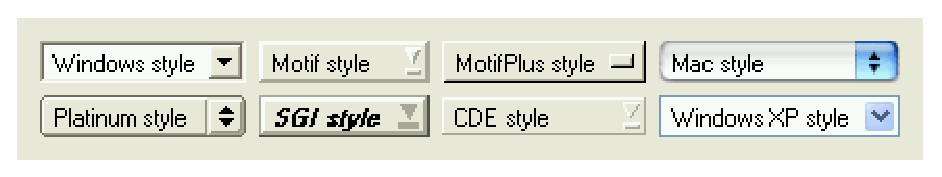
\includegraphics[scale=0.75,width=8.5cm]{pics/combobox.ps}
			}
	\end{itemize}

\end{slide}


%%%%%%%%%%%%%%%%%%%%%%%%%%%%%%%%%%%%%%%%%%%%%%%%%%%%%%%%%%%%%%%%%%%%%%%%%%%%%%%
%% SLIDE

\begin{slide}{Was ist Qt?}

	\begin{itemize}
		\item Editionen und Lizenzrecht
			{\small
			\begin{itemize}
				\item Kommerziell: Professional und Enterprise Edition 
				\item Nicht-kommerziell: Free Edition (QPL/GPL)
			\end{itemize}
			}
		\item Prominentestes Beispiel: KDE
			{\center
				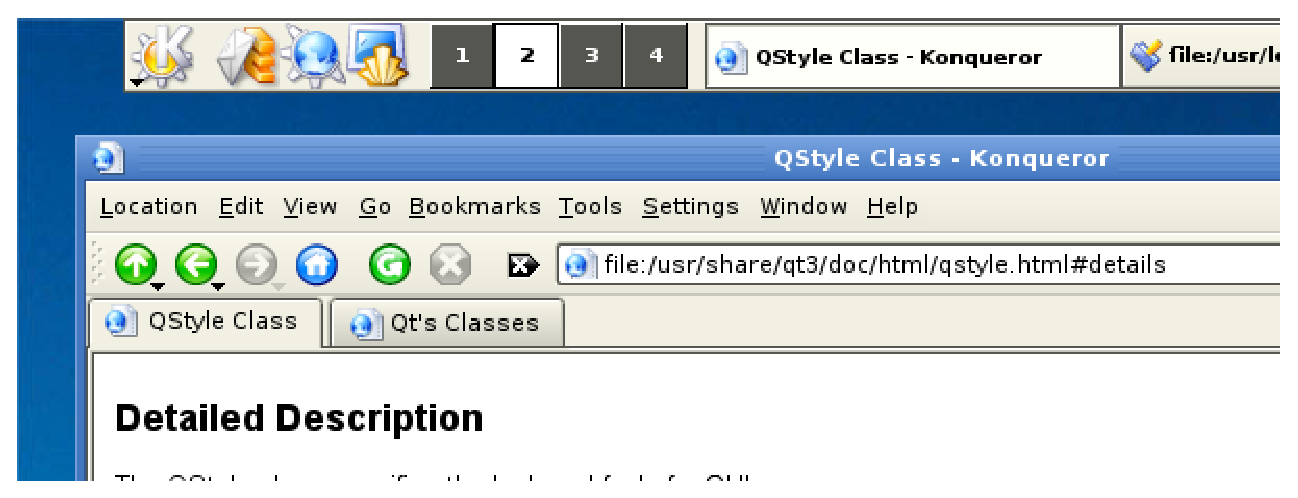
\includegraphics[scale=0.75,width=8.5cm]{pics/kde-desktop.ps}
			}
\end{itemize}

\end{slide}

%%%%%%%%%%%%%%%%%%%%%%%%%%%%%%%%%%%%%%%%%%%%%%%%%%%%%%%%%%%%%%%%%%%%%%%%%%%%%%%
%% SLIDE

\begin{slide}{Motivation}

	\begin{itemize}
		\item Portabilit�t
		\item Reduzierung des Entwicklungsaufwands (Kosten)
					f�r GUI Applikationen
		\item C++
			{\small
			\begin{itemize}
				\item Hohe Akzeptanz
				\item Hohe Performance
				\item Hoher Verbreitungsgrad (Mitte 90er)
				\item Objektorientierung
			\end{itemize}
			}
	\end{itemize}

\end{slide}


%%%%%%%%%%%%%%%%%%%%%%%%%%%%%%%%%%%%%%%%%%%%%%%%%%%%%%%%%%%%%%%%%%%%%%%%%%%%%%%
%% SLIDE

\begin{slide}{Architektur}

	\begin{itemize}
		\item Grundlegende Architektur:
		{\center
			\includegraphics[scale=0.75,width=8.5cm]{pics/architecture-diag.ps}
		}
		\item MVC Konzept (Model-View-Controller)
		\item Baumartige Klassenstruktur
		\item Neuartiges Event-Handling (Signals/Slots)
	\end{itemize}
\end{slide}


%%%%%%%%%%%%%%%%%%%%%%%%%%%%%%%%%%%%%%%%%%%%%%%%%%%%%%%%%%%%%%%%%%%%%%%%%%%%%%%
%% SLIDE
%%

\begin{slide}{Klassenhierarchie}
	\vspace*{-13pt}
	{\center
		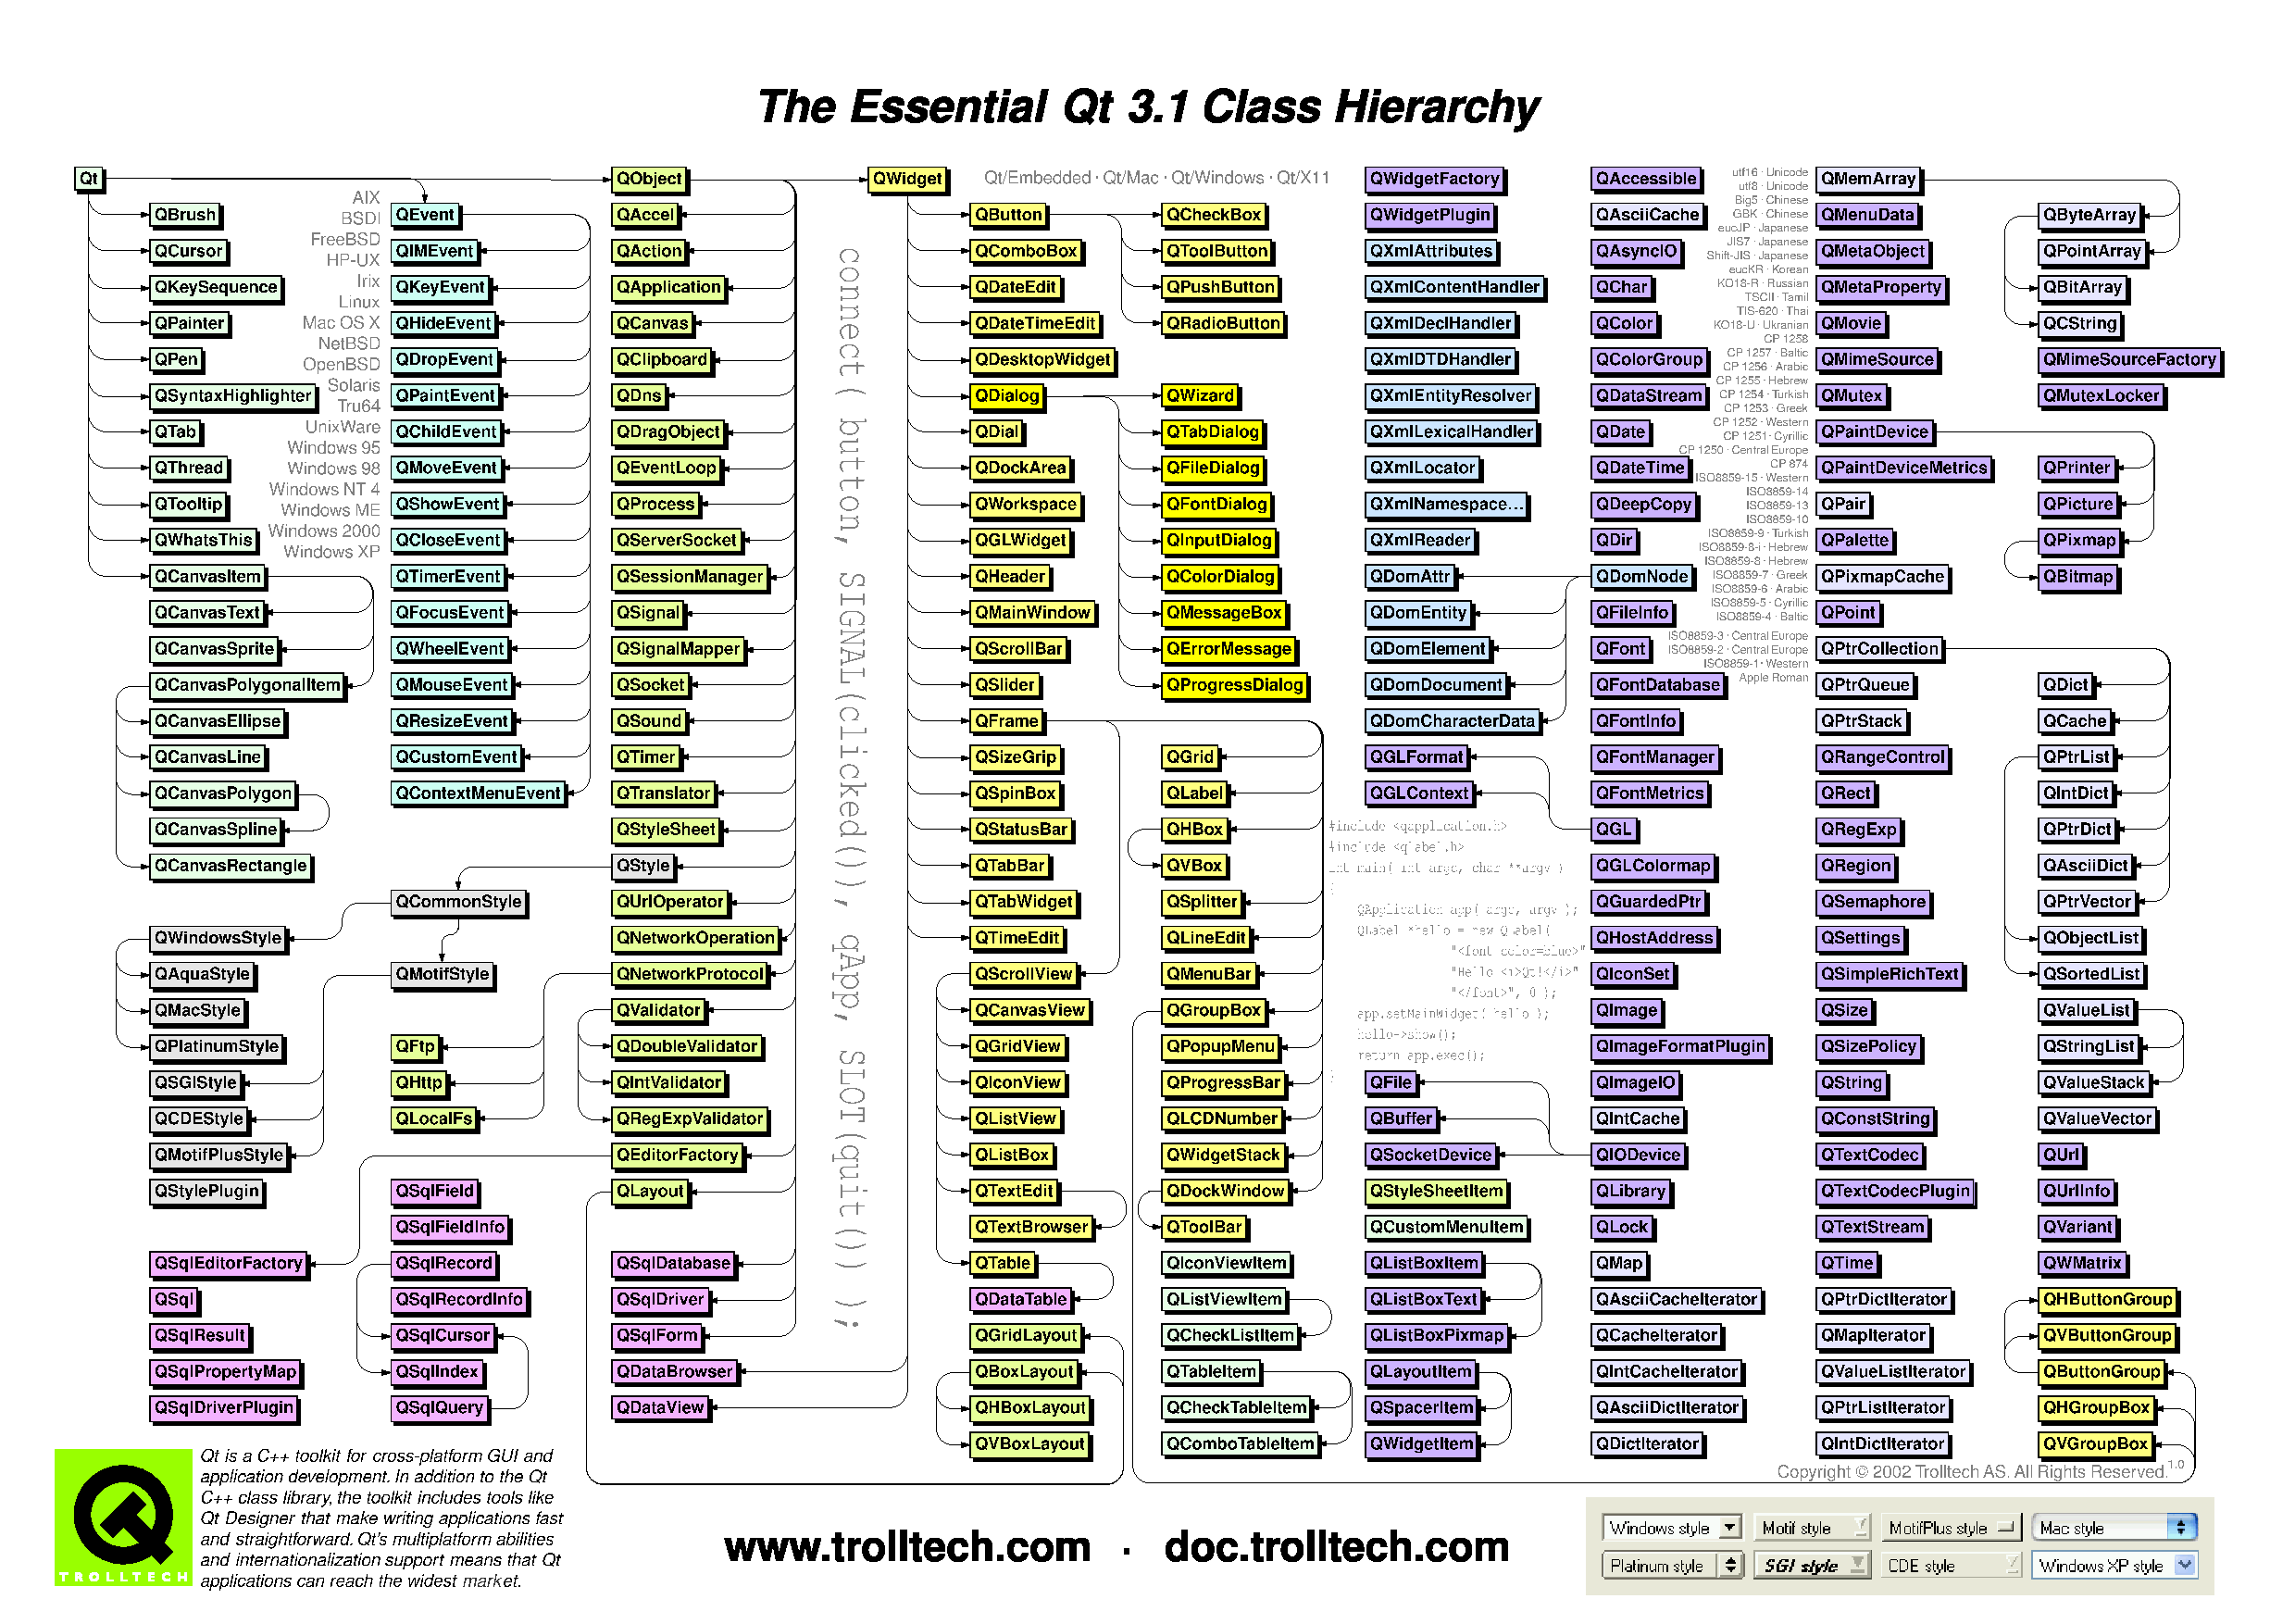
\includegraphics[scale=0.75,width=10.3cm]{pics/classchart.ps}
	}
\end{slide}

%%%%%%%%%%%%%%%%%%%%%%%%%%%%%%%%%%%%%%%%%%%%%%%%%%%%%%%%%%%%%%%%%%%%%%%%%%%%%%%
%% SLIDE
%%

\begin{slide}{Widgets}
	\begin{itemize}
		\item Elemente einer GUI (Icons, Buttons, ...)
		\item Stellen Informationen dar
		\item Interagieren mit Benutzer und OS
	\end{itemize}
	{\center
		\includegraphics[scale=0.75,width=10.3cm]{pics/qwidget-diag.ps}
		{\tiny Ausschnitt aus QWidget Klassenhierarchie}
	}
\end{slide}

%%%%%%%%%%%%%%%%%%%%%%%%%%%%%%%%%%%%%%%%%%%%%%%%%%%%%%%%%%%%%%%%%%%%%%%%%%%%%%%
%% SLIDE
%%

\begin{slide}{Layout}
	\vspace*{-13pt}
	{\center
		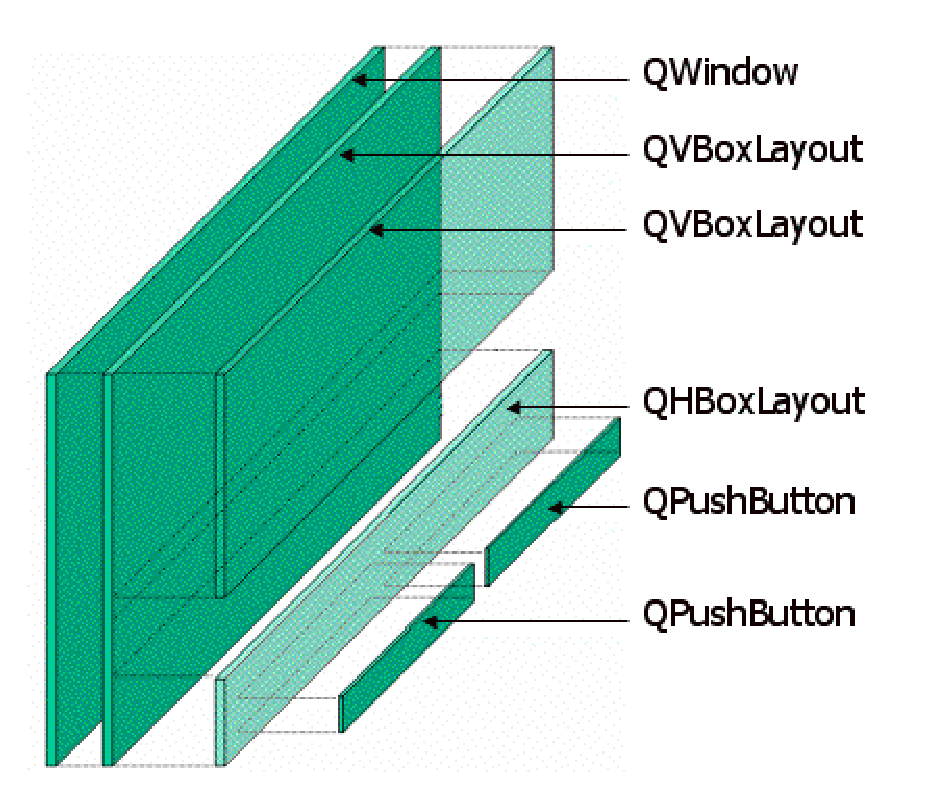
\includegraphics[scale=0.75,width=8cm]{pics/layout.ps}
	}
\end{slide}


%%%%%%%%%%%%%%%%%%%%%%%%%%%%%%%%%%%%%%%%%%%%%%%%%%%%%%%%%%%%%%%%%%%%%%%%%%%%%%%
%% SLIDE
%%

\begin{slide}{Hello Qt Beispiel}
	\lstset{language=c++}
	\lstset{commentstyle=\textit}
	\lstset{basicstyle=\tiny}
	\lstset{numbers=left}
	\begin{lstlisting}{}
#include <qapplication.h>
#include <qlabel.h>

int main( int argc, char **argv )
{
    QApplication app( argc, argv );
    QLabel *hello = new QLabel( "<font color=blue>Hello <i>Qt!</i>"
                                "</font>", 0 );
    app.setMainWidget( hello );
    hello->show();
    return app.exec();
}
\end{lstlisting}
\end{slide}


%%%%%%%%%%%%%%%%%%%%%%%%%%%%%%%%%%%%%%%%%%%%%%%%%%%%%%%%%%%%%%%%%%%%%%%%%%%%%%%
%% SLIDE
%%

\begin{slide}{Hello Qt Beispiel}
		{\center
			\includegraphics[scale=0.75,width=5cm]{pics/hello.ps}
		}
\end{slide}


%%%%%%%%%%%%%%%%%%%%%%%%%%%%%%%%%%%%%%%%%%%%%%%%%%%%%%%%%%%%%%%%%%%%%%%%%%%%%%%
%% SLIDE
%%

\begin{slide}{QApplication}

	\begin{itemize}
		\item Zentrales Objekt einer Qt Applikation
		\item Verwaltet Event-Kommunikation mit dem OS
		\item Enth�lt Event Loop
		\item Verantwortlich f�r Look \& Feel
		\item Verwaltet Lokalisierungs Unterst�tzung 
		\item Analysiert Kommandozeilenargumente
		\item �ber implizites {\it qApp} Objekt global verf�gbar
	\end{itemize}
\end{slide}

%%%%%%%%%%%%%%%%%%%%%%%%%%%%%%%%%%%%%%%%%%%%%%%%%%%%%%%%%%%%%%%%%%%%%%%%%%%%%%%
%% SLIDE
%%

\begin{slide}{Signal/Slot Konzept}
	\vspace*{-6pt}
	\begin{itemize}
		\item Zentrales Event-Handling in Qt Applikationen
		\item Signal:\\
					{\small Ausl�ser f�r eine Aktion}
		\item Slot:\\
					{\small Signalempf�nger, der die Aktion ausf�hrt}
		\item Verkn�pfung �ber {\it connect()} Methode
		\item Beliebig viele Signals und Slots pro Klasse
		\item Mehrfachverk�pfung m�glich
		\item Eigene Signals und Slots m�glich
	\end{itemize}
\end{slide}

%%%%%%%%%%%%%%%%%%%%%%%%%%%%%%%%%%%%%%%%%%%%%%%%%%%%%%%%%%%%%%%%%%%%%%%%%%%%%%%
%% SLIDE
%%

\begin{slide}{Signal/Slot Konzept (abstrakt)}
	\vspace*{-10pt}
		{\center
			\includegraphics[scale=0.75,width=7cm]{pics/abstract-connections.ps}
		}
\end{slide}

%%%%%%%%%%%%%%%%%%%%%%%%%%%%%%%%%%%%%%%%%%%%%%%%%%%%%%%%%%%%%%%%%%%%%%%%%%%%%%%
%% SLIDE
%%

\begin{slide}{Signal/Slot Konzept (konkret)}
		{\center
			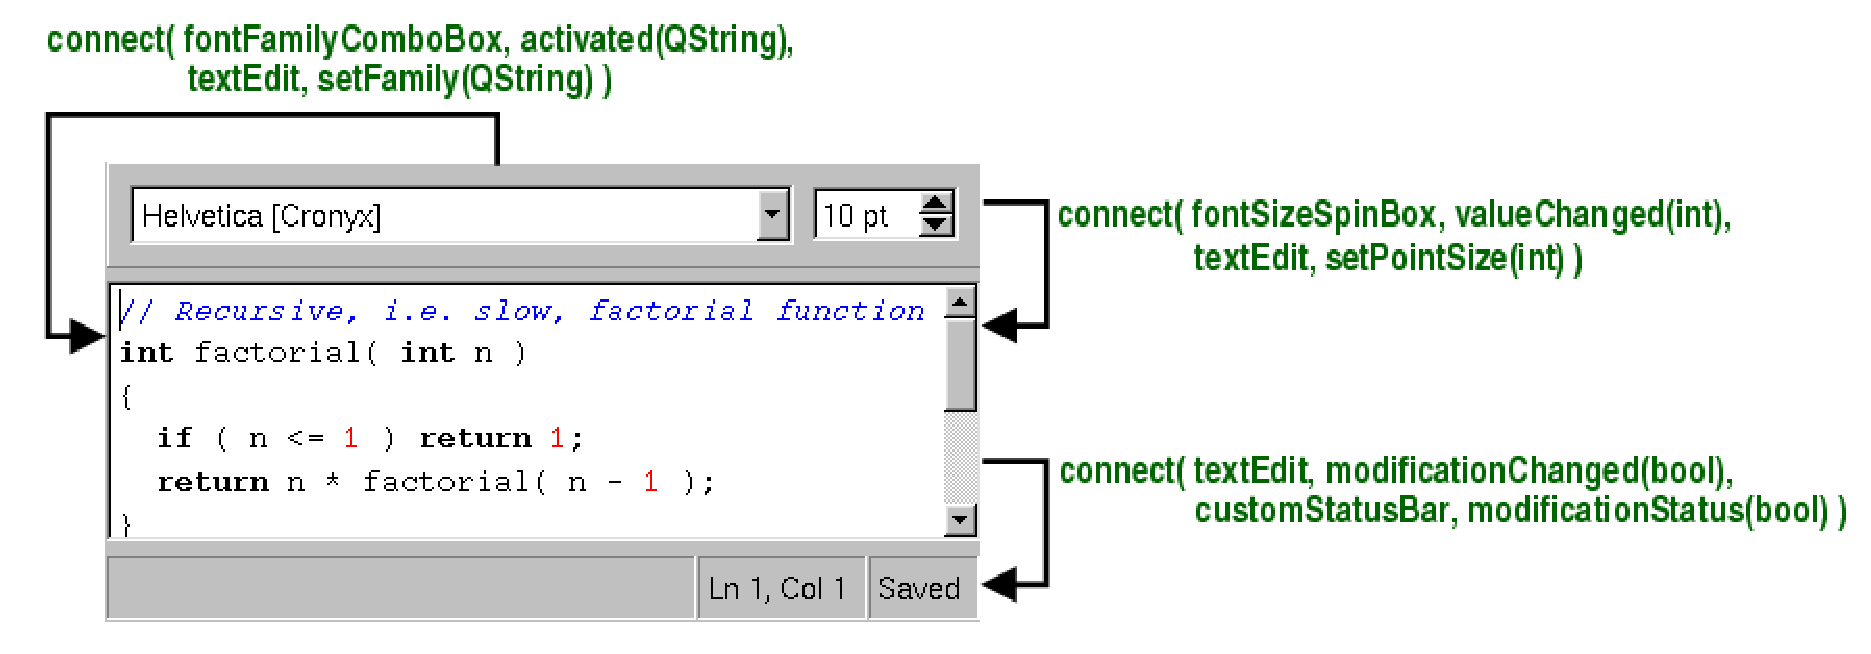
\includegraphics[scale=0.75,width=11.5cm]{pics/concrete-connections.ps}
		}
\end{slide}

%%%%%%%%%%%%%%%%%%%%%%%%%%%%%%%%%%%%%%%%%%%%%%%%%%%%%%%%%%%%%%%%%%%%%%%%%%%%%%%
%% SLIDE
%%

\begin{slide}{Signal/Slot Konzept (Code)}
	\begin{itemize}
		\item Eigene Signals und Slots werden in Header-Datei definiert
	\lstset{language=c++}
	\lstset{commentstyle=\textit}
	\lstset{basicstyle=\tiny}
	\lstset{numbers=left}
	\begin{lstlisting}{}
class BlaFasel : public QMainWindow {

    O_OBJECT    // WICHTIGES MACRO!!!
...
signals:
    void text(const QString&);
public slots:
protected slots:
private slots:
    void newFile();
\end{lstlisting}
	\end{itemize}
\end{slide}

%%%%%%%%%%%%%%%%%%%%%%%%%%%%%%%%%%%%%%%%%%%%%%%%%%%%%%%%%%%%%%%%%%%%%%%%%%%%%%%
%% SLIDE
%%

\begin{slide}{Signal/Slot Konzept}
	\begin{itemize}
		\item Wichtig: {\it Q\_OBJECT} Macro einbinden bei eigenen Signalen
		\item Meta Object Compiler (MOC) dient als Preprocessor zur
					Verarbeitung von Signals und Slots Definitionen
		\item MOC generiert {\it moc\_*.cpp} Dateien
		\item Signal-{\it member}-Funktionen werden nur(!) vom MOC erzeugt
		\item Slot-{\it member}-Funktionen werden ganz normal implementiert
	\end{itemize}
\end{slide}

%%%%%%%%%%%%%%%%%%%%%%%%%%%%%%%%%%%%%%%%%%%%%%%%%%%%%%%%%%%%%%%%%%%%%%%%%%%%%%%
%% SLIDE
%%

\begin{slide}{Signal/Slot Konzept - connect()}
	\lstset{language=c++}
	\lstset{commentstyle=\textit}
	\lstset{basicstyle=\tiny}
	\lstset{numbers=left}
	\begin{lstlisting}{}
#include "blafasel.h"

BlaFasel::BlaFasel(QWidget* parent, const char *name, WFlags f) :
    QMainWindow(parent, name, f)
{
...
    blubber = new QAction("New File", QPixmap(filenew), "&New", ...);
...
    connect(blubber, SIGNAL(text(const QString&)),
            this, SLOT(newFile()));
...
}
\end{lstlisting}
\end{slide}

%%%%%%%%%%%%%%%%%%%%%%%%%%%%%%%%%%%%%%%%%%%%%%%%%%%%%%%%%%%%%%%%%%%%%%%%%%%%%%%
%% SLIDE
%%

\begin{slide}{Tools - qmake}
	\begin{itemize}
		\item Generiert plattformspezische Makefile aus einer
					{\it <project>.pro} Datei
		\item Startet Meta Object Compiler zur Signal/Slot Verarbeitung
		\item Sollte nach jeder Signal/Slot �nderung aufgerufen werden
		\item Sollte vor jeder Portierung aufgerufen werden
		\item Aufruf: {\it qmake -o Makefile <project>.pro}
	\end{itemize}
\end{slide}

%%%%%%%%%%%%%%%%%%%%%%%%%%%%%%%%%%%%%%%%%%%%%%%%%%%%%%%%%%%%%%%%%%%%%%%%%%%%%%%
%% SLIDE
%%

\begin{slide}{Tools - qmake - sample.pro}
	\lstset{language=make}
	\lstset{commentstyle=\textit}
	\lstset{basicstyle=\small}
	\lstset{numbers=left}
	\begin{lstlisting}{}
TEMPLATE	= app
CONFIG		+= qt warn_on release thread
HEADERS		= sample.h
SOURCES		= sample.cpp main.cpp
TARGET		= sample 
\end{lstlisting}
\end{slide}

%%%%%%%%%%%%%%%%%%%%%%%%%%%%%%%%%%%%%%%%%%%%%%%%%%%%%%%%%%%%%%%%%%%%%%%%%%%%%%%
%% SLIDE
%%

\begin{slide}{Tools - Qt Designer}
	\begin{itemize}
		\item Bietet grafische Erstellung (per Drag \& Drop) 
					von dialogbasierten Layouts an
		{\center
			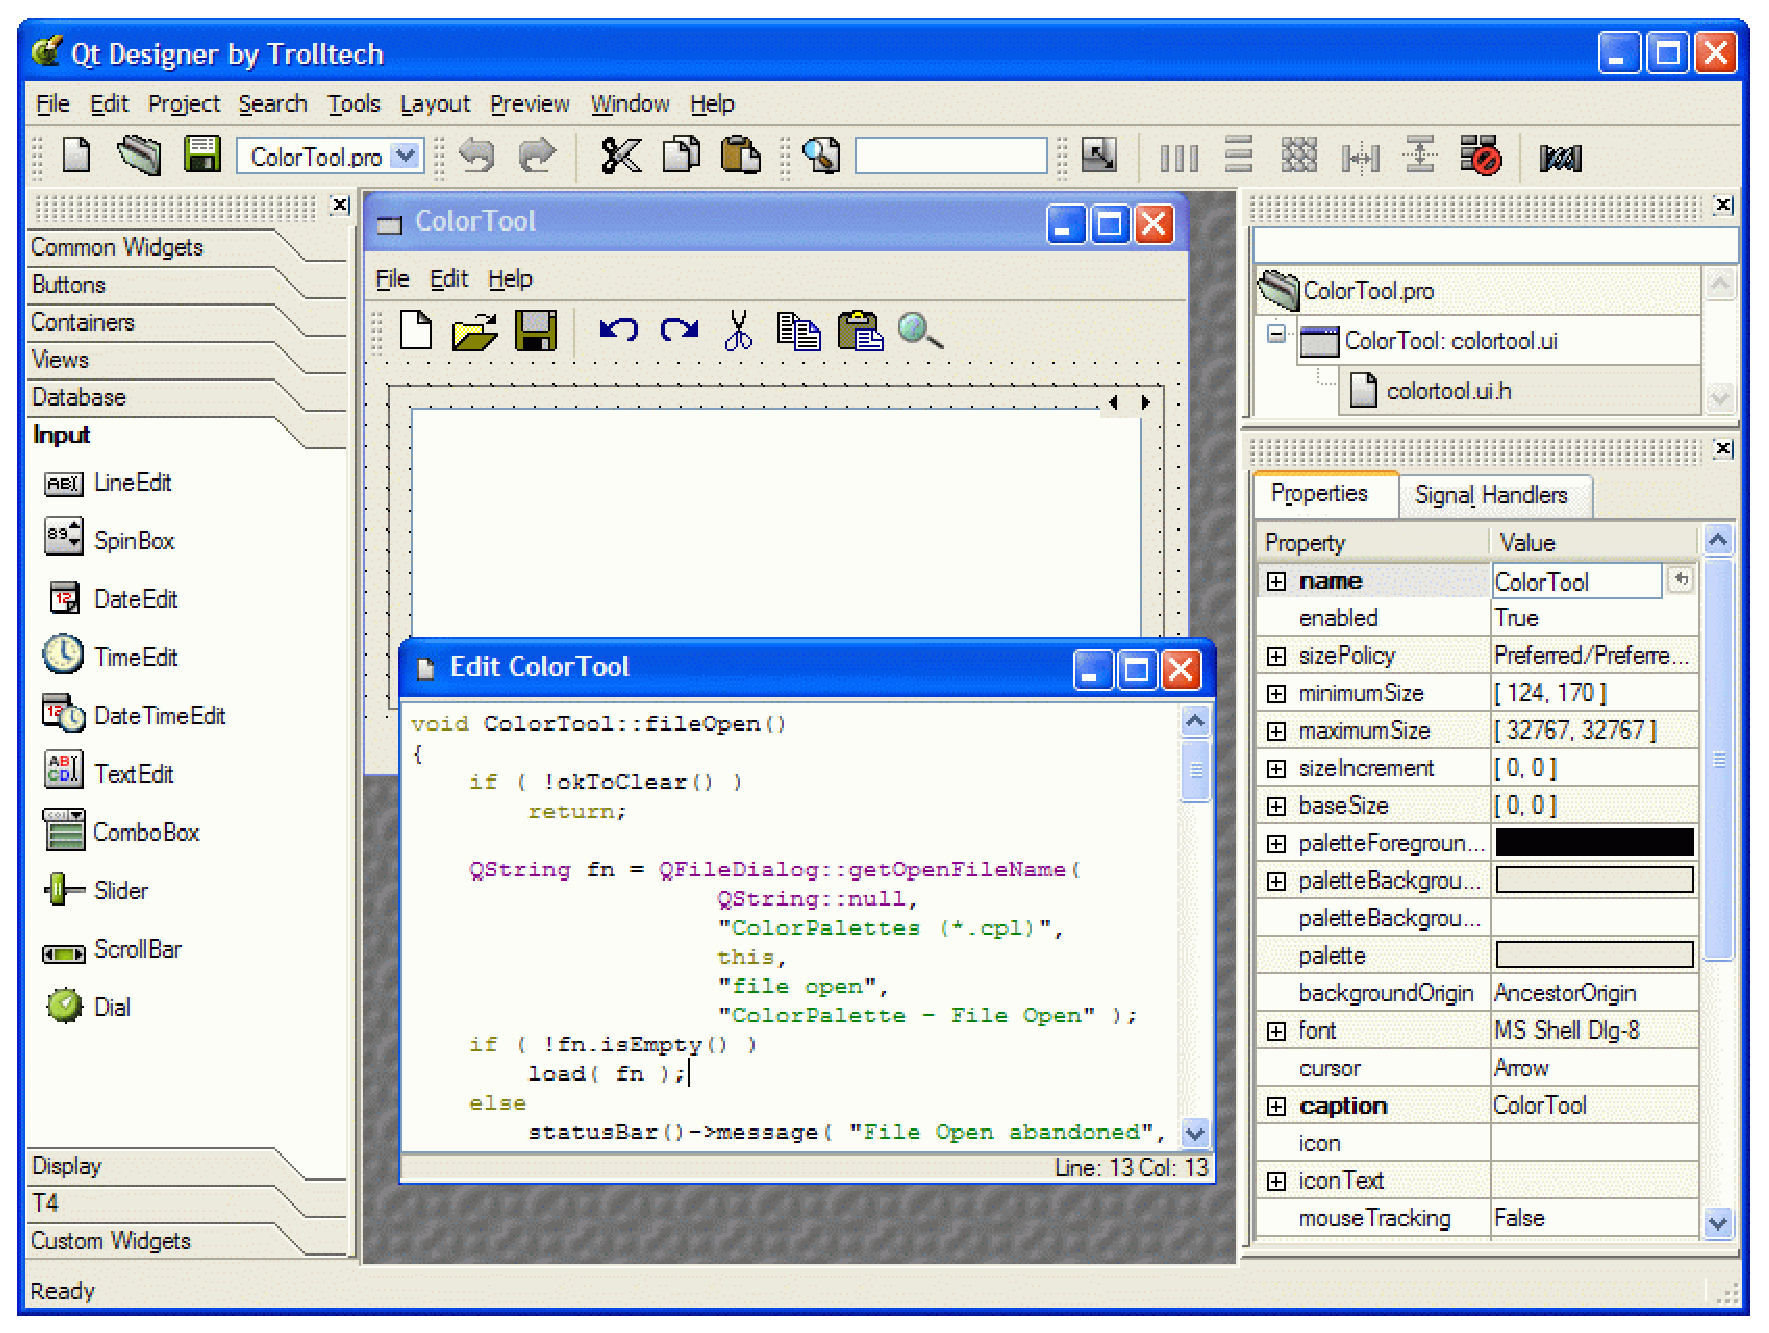
\includegraphics[scale=0.75,width=7cm]{pics/designer.ps}
		}
	\end{itemize}
\end{slide}

%%%%%%%%%%%%%%%%%%%%%%%%%%%%%%%%%%%%%%%%%%%%%%%%%%%%%%%%%%%%%%%%%%%%%%%%%%%%%%%
%% SLIDE
%%

\begin{slide}{Tools - Qt Designer}
	\begin{itemize}
		\item Umfasst alle wesentlichen Widgets
		\item Unterst�tzt Signal/Slot Konzept
		\item Enth�lt Source Code Editor
		\item Erzeugt XML-basierte Ressourcendatei, die mit {\it uic}
				in C++ Code �bersetzt wird
		\item Unterst�tzt keine R�ck�bersetzung
		\item Unterst�tzt kein MDI
	\end{itemize}
\end{slide}


%%%%%%%%%%%%%%%%%%%%%%%%%%%%%%%%%%%%%%%%%%%%%%%%%%%%%%%%%%%%%%%%%%%%%%%%%%%%%%%
%% SLIDE
%%

\begin{slide}{Quellen und weiterf�hrende Lekt�re}
	\begin{itemize}
		\item Borkner-Delcarlo, Olaf, "GUI-Programmierung mit Qt"
					(Hanser Verlag 2002)
		\item http://doc.trolltech.com
		\item Empfehlung:\\ {\small
ftp://ftp.trolltech.com/qt/pdf/3.1/qt-whitepaper-a4-web.pdf}
	\end{itemize}
\end{slide}

\end{document}
